\chapter{Confronto tra le implementazioni}
Nel corso degli ultimi anni la community di sviluppatori ha portato avanti diverse iniziative per imporre uno standard condiviso per le security token offering. Inizialmente lo standard de facto è stato ERC-20\cite{K37}, già ampiamente adottato dalla maggior parte delle Initial coin Offering. Tra gli standard utilizzati per le STO, ERC-20 è lo standard più maturo e con maggiore supporto essendo stato creato verso la fine del 2015. Altri tentativi di standardizzazione nascono dalla necessità di garantire all'issuer della security token offering una maggiore governance e per facilitare il rispetto delle regolamentazioni sulle securities. Non a caso infatti possiamo osservare come molti tentativi di standardizzazione siano stati operati da aziende che offrono piattaforme per il token issuing. Per la maggior parte di queste aziende l'approccio è stato quello di estendere lo standard ERC-20, in modo da ottenere retrocompatibilità ed essere più appetibili alla community di sviluppatori con conoscenza dello standard sopracitato. Tra i casi che verranno analizzati troviamo: 
\begin{itemize}
    \item ST-20\cite{K38}, sviluppato da Polymath
    \item R-Token\cite{K39}, sviluppato da Harbor
    \item DS Protocol\cite{K41}, sviluppato da Securitize
    \item T-REX\cite{K42}, sviluppato da Tokeny
    \item S3\cite{K43}, sviluppato da OpenFinace
\end{itemize}

Altri standard si sono sviluppati a partire da necessità diverse, come nel caso degli standard ERC-721 ed ERC-1155 che implementano token non fungibili. La notorietà di questi protocolli è in parte dovuta all'introduzione del concetto di scarsità digitale tramite l'utilizzo di token non omogenei, un approccio che ben si presta all'ambito videoludico. 
Una proposta più recente e che ha ottenuto maggiore supporto sia dalla community sia da aziende, alcune delle quali già in possesso di uno standard proprietario, è lo standard ERC-1400, rinominato Security Token Standard\cite{K45}. ERC-1400 è una collezione di diversi standard sviluppati per essere interoperabili e facilmente estendibili all'emergere della necessità di nuove funzionalità da introdurre. Il passaggio ad uno standard condiviso e supportato da più stakeholder rappresenta uno step fondamentale par la diffusione di questo fenomeno.

\section{Implementazione con token ERC-20}
ERC-20 definisce un'interfaccia standard che rappresenta un token. Lo standard fornice funzionalità basilari per il trasferimento dei token. Lo scopo principale dello standard è quello di permettere interoperabilità tra le applicazioni che supportano lo standard, come ad esempio wallets ed exchanges. 
Lo standard ERC-20 prevede le seguenti funzioni:
\begin{lstlisting}[language=Solidity,numbers=none]
totalSupply() public view returns (uint256 totalSupply)
\end{lstlisting} 
\begin{lstlisting}[language=Solidity,numbers=none]
balanceOf(address _owner) public view returns (uint256 balance)\end{lstlisting}
\begin{lstlisting}[language=Solidity,numbers=none] 
transfer(address _to, uint256 _value) public returns (bool success)\end{lstlisting} 
\begin{lstlisting}[language=Solidity,numbers=none]
transferFrom(address _from, address _to, uint256 _value) public returns (bool success)
\end{lstlisting}
\begin{lstlisting}[language=Solidity,numbers=none]
approve(address _spender, uint256 _value) public returns (bool success)
\end{lstlisting}
\begin{lstlisting}[language=Solidity,numbers=none]
allowance(address _owner, address _spender) public view returns (uint256 remaining)
\end{lstlisting}
Inoltre, vengono definiti i seguenti eventi:
\begin{lstlisting}[language=Solidity,numbers=none]
Transfer(address indexed _from, address indexed _to, uint256 _value)
\end{lstlisting}
\begin{lstlisting}[language=Solidity,numbers=none]
Approval(address indexed _owner, address indexed _spender, uint256 _value)
\end{lstlisting}
Due delle implementazioni più diffuse di questo standard sono state realizzate da OpenZeppelin e ConsenSys. Le due implementazioni sono entrambe pienamente compatibili con lo standard sebbene presentino delle lievi differenze come si può osservare in appendice \ref{appendix:ERC-20Interface}.

Una appunto interessante si può trarre osservando i cambiamenti avvenuti durante lo sviluppo iniziale dello standard. Se in principio le prime bozze dello standard prevedevano un focus sulla creazione di "Coin", gli sviluppatori in modo lungimirante hanno deciso di generalizzare il protocollo per renderlo applicabile ad ogni bene fungibile trasferibile, motivo per il quale è stata scelta la denominazione più generica di "token"\cite{https://www.reddit.com/r/ethereum/comments/3n8fkn/lets_talk_about_the_coin_standard/}.

\subsection{ERC-20 proprietary extension}
\subsubsection{ST-20}
Lo standard ST-20 introdotto da Polymath nasce con l'obbiettivo di aggiungere all'interfaccia ERC20 la possibilità di inserire restrizioni allo scambio di token in modo da poter essere conforme alle normative sulle securities. 
In appendice \ref{appendix:ST20} è possibile osservare l'interfaccia dello smart contract che definisce un security token che rispetta lo standard ST-20. Trattandosi di un'estensione, lo smart contract è compatibile con lo standard ERC-20 e ne implementa tutte le funzioni e gli eventi previsti, aggiungendo a questi altre funzionalità e caratteristiche che agevolano l'adattabilità e la governance della STO. Per esempio, nel caso dello scambio senza restrizioni tra due parti, un caso che non sempre è desiderabile nelle STO, le transazioni possono essere limitare da una funzione "verifyTransfer". Ciò permette inoltre l'implementazione di una whitelist, una blacklist, un limite minimo/massimo di trasferimento, etc. 
In modo più dettagliato, l'interfaccia creata da Polymath si avvale principalmente di tre tipi componenti: un primo tipo detto "Transfer Manager", un tipo di moduli denominati "permission modules" e infine un modulo che si occupa delle funzionalità della token sale, ovvero, gli "STO modules". 
L'utilizzo di numerose componenti per implementare diverse funzionalità permette di avere un architettura modulare che comprende di volta in volta solamente le funzionalità richieste, permettendo così di rendere lo smart contract più efficiente.

\subsubsection{R-Token}
R-token, implementat da Harbor offre delle caratteristiche che lo rendono particolarmente innovativo, tanto da essere concettualmente compatibile con un token ERC-1400.Un altro aspetto particolare del protocollo è l'integrazione di una whitelist per gli exchange presenti nell'ecosistema proposto da Harbor. 
R-Token, che sta per "regualted token" si differenzia dagli altri standard compatibili con ERC-20 D<per l'adozione di alcuni servizi di document management e di custody. 
Generalmente una STO Harbor si compone di tre smart contracts;
\begin{itemize}
    \item Un "Regulator Service" che si occupa di interagire tramite un oracolo con la regolamentazione definita off.chain. 
    \item Un "Service Registry" che contiene un riferimento al "Regulator Service". Questo riferimento può essere modificato per permettere di aggiornare la business logic della STO. 
    \item Uno smart contract "R-Token" che contiene le caratteristiche del token, le sue funzioni e un riferimento immutabile al "Service Registry"
\end{itemize}
\subsubsection{DS Protocol}
L'estensione di ERC-20 proposta da Securitize ha due componenti principali. Il primo è lo smart contract "DSTokenInterface" che nel complesso non risulta apportare cambiamenti rilevanti rispetto ai protocolli già presentati. Il secondo componente risulta essere più originale ed è lo smart contract "DSServiceConsumerInterface" definito come segue:
\begin{lstlisting}[language=Solidity,numbers=none]
function getDSService(uint _serviceId) public view returns (address);

function setDSService(uint _serviceId, address _address) public /*onlyMaster*/ returns (bool);
\end{lstlisting}
queste funzioni permettono l'associazione dinamica di componenti e di verificare la presenza componenti  in modo dinamico (al fine di mantenere compatibilità tra diverse versioni del protocollo). I servizi sono identificati da un id nel seguente modo:
\begin{lstlisting}[language=Solidity,numbers=none]
 uint public constant TRUST_SERVICE = 1;
 uint public constant DS_TOKEN = 2;
 uint public constant REGISTRY_SERVICE = 4;
 uint public constant COMPLIANCE_SERVICE = 8;
 uint public constant COMMS_SERVICE = 16;
 uint public constant WALLET_MANAGER = 32;
 uint public constant LOCK_MANAGER = 64;
 uint public constant ISSUANCE_INFORMATION_MANAGER = 128;
 \end{lstlisting}
\subsubsection{T-REX}
T-REX, per esteso "Token for Regulated EXchanges", Presenta un approccio diverso rispetto ad altri protocolli. L'identità infatti ricopre un ruolo fondamentale nel protocollo, tanto da prevedere dei meccanismi di gestione dell'identità dell'investitore on-chain secondo i protocolli ERC-725 ed ERC-735. Il meccanismo di controllo dell'identità sostituisce la logica di whitelisting e blacklisting rendendo il protocollo più flessibile. Possiamo osservare il funzionamento del protocollo nel seguente diagramma in figura \ref{fig:trex}.
\begin{figure}[H]
  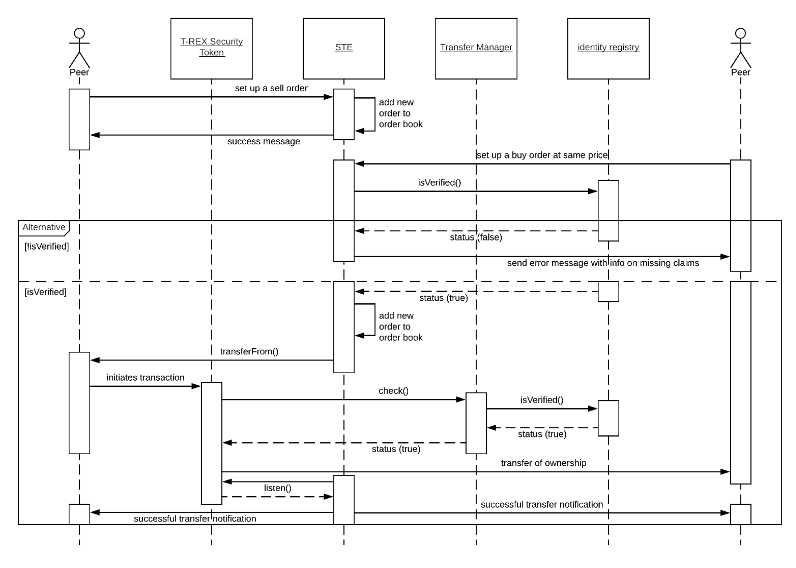
\includegraphics[width=\linewidth]{trex.png}
  \caption{Sequence diagram of a Distributed Security Token Exchange  transaction with T-REX tokens}
  \label{fig:trex}
\end{figure}
\subsubsection{S3}
S3, per esteso Smart Securities Standard, è un altra estensione di ERC-20 che si distingue per una semplice caratteristica di compliance. Infatti Il protocollo S3 include degli smart contract dedicati ad implementare le restrizioni e le regole imposte dalla Regulation D, la Regulation S, la Regulation A+ e Regulation CF.

\begin{lstlisting}[language=Solidity,numbers=none]
///RegD506c.sol
/// @title Functions that tokens will need to call to configure themselves 
contract RegD506c is TransferRestrictor {
  function startHoldingPeriod() public;
  function registerAmlKycChecker(address _checker, address _token) public;
  function registerAccreditationChecker(address _checker, address _token) public;
}
\end{lstlisting}

Questo approccio semplifica notevolmente la struttura del protocollo ma presenta numerosi svantaggi, soprattutto in termini di manutenibilità. Nell'ultima versione disponibile del protocollo l'approccio è mutato notevolmente, tanto che la restrizione degli scambi è delegata ad un altro smart contract non specificato. 
\section{Implementazione con token ERC-721 e ERC-1155}
Sebbene non siano pensati in modo specifico per le securities, gli standard ERC-721 ed ERC-1155 sono rilevanti per l'argomento analizzato in quanto permettono di tokenizzare assets fisici. Tramite l'introduzione del concetto di non fungibilità nello standard ERC-721 infatti è possibile definire uno smart contract in cui un token è unico. Questo concetto si può applicare con facilità ad oggetti rari, unici oppure ogni tipo di oggetto collezionabile. La sua implementazione più famosa è il progetto CryptoKitties, un gioco che permette di comprare, vendere e scambiare carte virtuali. nel 2017 il gioco divenne talmente popolare da congestionare la rete Ethereum. Ogni carta rappresenta un CryptoKitty, ovvero un token  non-fungibile. Ad oggi sono stati scambiati Cryptokitties per un valore superiore a 27 milioni di dollari. Il valore di un singolo token può raggiungere cifre molto alte e sono nati exchange dedicati a questo protocollo, come possiamo vedere in figura \ref{figure:kitty}.
\begin{figure}[H]
  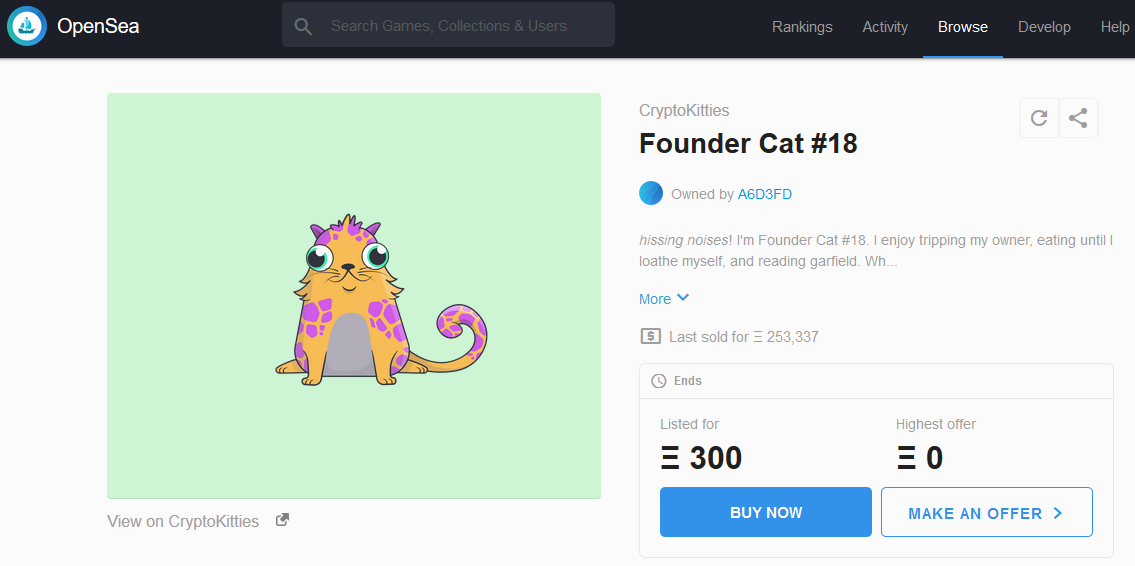
\includegraphics[width=\linewidth]{kitty.png}
  \caption{Second most expensive CryptoKitty, traded on a specialized exchange}
  \label{fig:kitty}
\end{figure}
ERC-1155 rappresenta un evoluzione dei token ERC-20 ed ERC-721, poiché permette di gestire sia token fungibili che non fungibili in un unico contratto, permettendo transazioni con più token di tipo diverso. Questa funzionalità è stata realizzata con l'obbiettivo di permettere l'adozione di token in videogiochi più complessi rispetto a CryptoKitties, come nel caso di giochi che permetto la vendita, l'acquisto e lo scambio di una currency del gioco e di oggetti virtuali. 

\section{Implementazione con token ERC-1400}
https://github.com/ConsenSys/ERC1400
https://blog.polymath.network/erc1400-implementation-approach-c668c4fbf40
https://github.com/bokkypoobah/SecurityToken
\subsection{ERC-1410: Partially Fungible Token Standard}
https://github.com/ethereum/EIPs/issues/1410
\subsection{ERC-1594: Core Security Token Standard}
https://github.com/ethereum/EIPs/issues/1594
\subsection{ERC-1643: Document Management Standard}
https://github.com/ethereum/EIPs/issues/1643
\subsection{ERC-1644: Controller Token Operation Standard}
https://github.com/ethereum/EIPs/issues/1644
\subsection{ERC-2258: Custodial Ownership Standard}
https://github.com/ethereum/EIPs/issues/2258
\section{Implementazione in altre blockchain}
\subsection{SRC20}
https://www.swarm.fund/src20
\subsection{Stellar}
https://medium.com/quillhash/ethereum-or-stellar-which-platform-is-best-suitable-for-your-ico-sto-7f1368bb942c
\subsection{EOS}
https://stoupdates.com/eos-enters-the-security-token-scene-with-the-launch-of-new-protocol/
\subsection{Hyperledger}
\subsection{Corda}
https://stowise.com/company/r3/
\subsection{Tezos}
https://www.reddit.com/r/tezos/comments/cdl2bu/tezos_explainer_3_reasons_why_tezos_is_the_best/
\subsection{NEO}
https://www.securities.io/neo-announces-formation-of-security-token-industry-consortium/
\subsection{Tron}
\section{Considerazioni sulle implementazioni}




https://info.binance.com/en/research/marketresearch/tokenization.html 



https://medium.com/atomic-capital/state-of-the-standards-a-technical-review-of-current-digital-securities-standards-3bc79f5aaf73
https://medium.com/@ElectricCapital/electric-capital-developer-report-h1-2019-7d836d68fecb